\section{RESULTS}
\subsection{CO EMISSIONS AND LINE RATIOS}

\begin{figure*}[htbp]
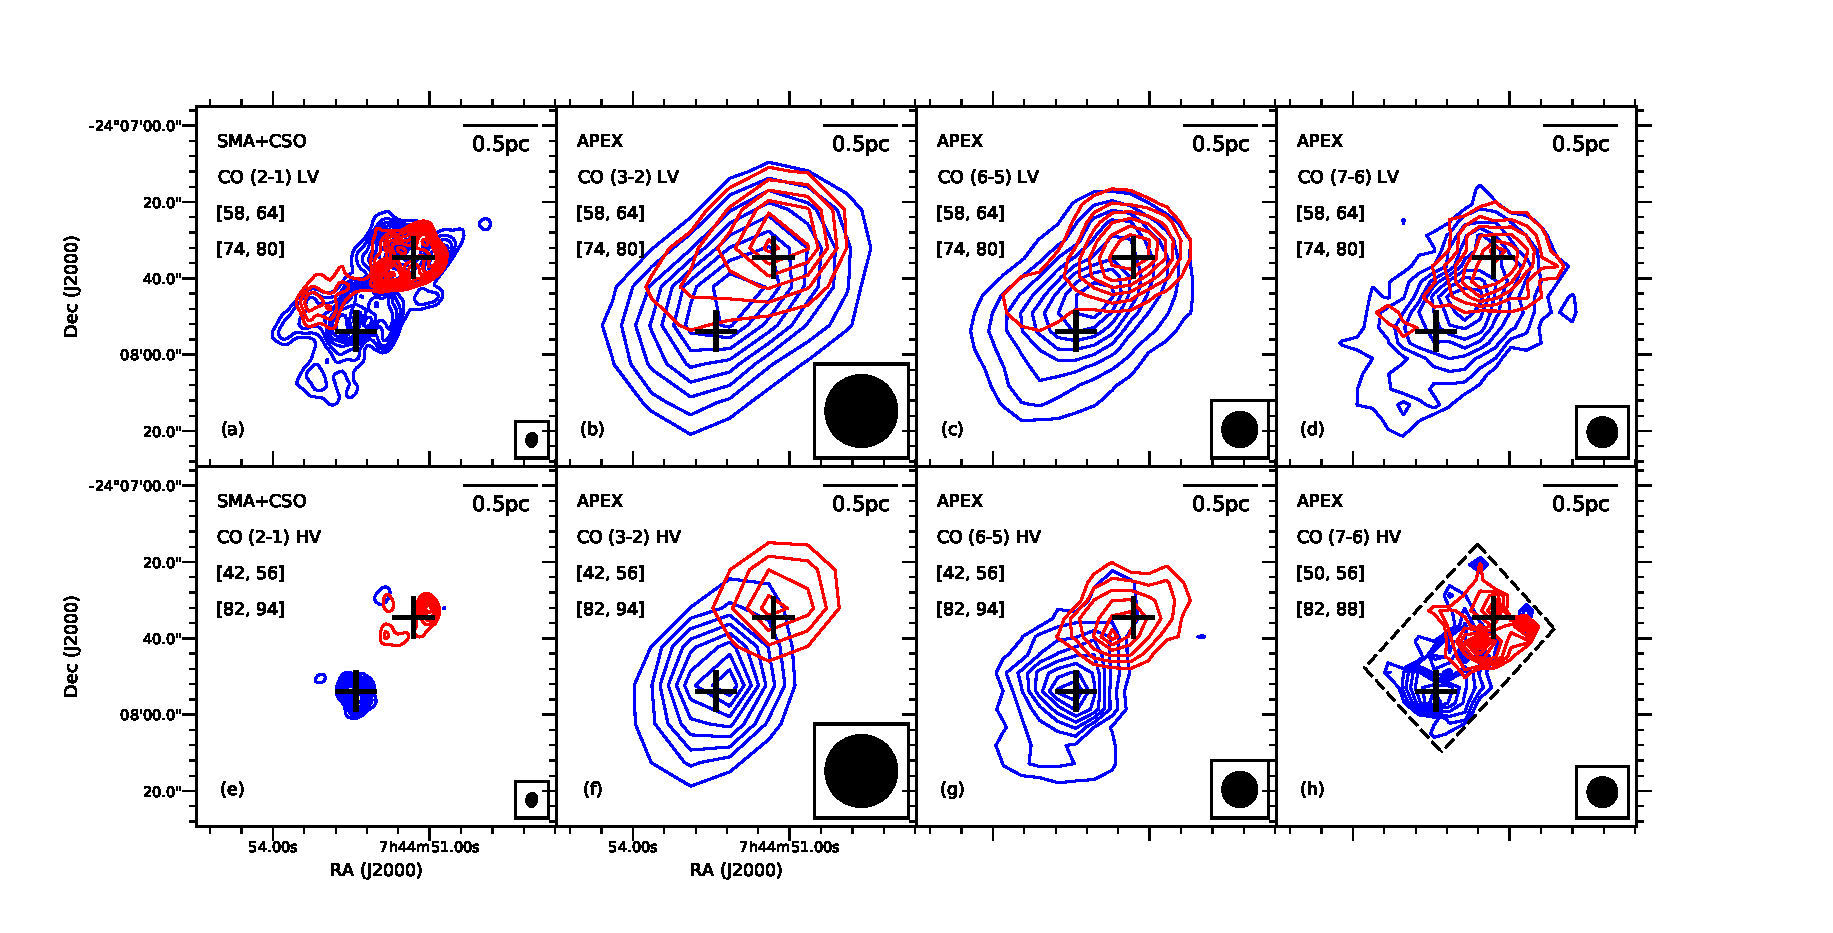
\includegraphics[scale=.60]{./fig/ori_contourall.eps}
\caption{(a)-(d) Low-velocity CO J = (2-1), (3-2), (6-5), (7-6) emissions, integrated from 58 to 64 km s$^{-1} $ for the blueshifted lobe (blue) and from 74 to 80 km s$^{-1}$ for the redshifted lobe (red); (e)-(g) High-velocity CO J = (2-1), (3-2), (6-5) emissions,  integrated from 42 to 56 km s$^{-1} $ for the blueshifted lobe (blue) and from 82 to 94 km s$^{-1}$ for the redshifted lobe (red); (h) High-velocity CO J = (7-6) emission, integrated from 50 to 56 km s$^{-1} $ for the blueshifted lobe (blue) and from 82 to 88 km s$^{-1}$ for the redshifted lobe (red). For (a)-(g), the contour levels start from 20\% and continue at steps of 10\% of the peak emission. For (h), the contour levels start from 30\% and continue at steps of 10\% of the peak emission. Data outside the dashed region are masked out because of the low signal-to-noise ratio. The beam size is shown in the lower right corner of each panel. The CO (2-1) maps are adopted from \citet{2009ApJ...696...66Q}. \label{fig1}}
\end{figure*}

The cloud velocity (v$_{\mathrm{cloud}}$) with respect to the local standard of rest is about 67.5 km s$^{-1}$, which is adopted from \citet{2003A&A...412..175K}. Figure \ref{fig1} shows the integrated low-velocity (LV) and high-velocity (HV) emissions of CO J = (2-1), (3-2), (6-5), (7-6). The outflow morphologies seen in CO (3-2), (6-5) and (7-6) are very similar. For the three lines detected by APEX, a prominent bipolar outflow at (PA) $\sim$ 131${\degr}$ along with a weaker component at PA $\sim$ 101${\degr}$ is detected. The weaker component is at relatively lower velocities, while the prominent component is detected at both low and high velocities. The signal-to-noise ratio in the CO (7-6) spectrum is relatively low at high velocities. Overall, the CO (3-2), (6-5), (7-6) maps presented in Figure \ref{fig1} are very similar to the CO (3-2) map presented by \citet{2003A&A...412..175K}. Due to angular resolution, the CO J = (3-2), (6-5), (7-6) emissions don't show the wide-angle structure highlighted by the CO (2-1) emission.

To compare the emissions of different CO transitions, we convolved the CO (2-1), (6-5) and (7-6) maps, to the same spatial resolution of the CO (3-2), which is 19${\arcsec}$. To reduce the noise level in the spectra, we resampled the four CO lines to a resolution of 2 km s$^{-1}$. Then we measured the main beam temperature ($T_{\mathrm{mb}}$) of different CO lines at the peak of the blueshifted and the redshifted lobes (marked as two crosses in each panel of Figure \ref{fig1}). Figure \ref{fig2} shows the observed line wing ratios of different CO transitions.  All line ratios in Figure \ref{fig2} are remarkably constant with velocity.

\begin{figure}[tbp]
\plotone{./fig/ratio.eps}
\caption{Ratios of the $T_{\mathrm{mb}}$ of different CO lines at different velocities. Blue symbols denote the measurements from the blueshifted lobe, and red symbols the redshifted lobe. The $V_{\mathrm{outflow}}$ shown here is related to the $v_{\mathrm{cloud}}$ by the relation: $V_{\mathrm{outflow}}$ = $\mid$ $v_{\mathrm{outflow}}$ - $v_{\mathrm{cloud}}\mid$, where $v_{\mathrm{outflow}}$ is the outflow velocity with respect to the local standard of rest. \label{fig2}}
\end{figure}

\subsection{PHYSICAL PROPERTY ANALYSIS}
Because the $^{13}$CO emission is not detected in the outflowing gas, the four transitions of $^{12}$CO are assumed to be optically thin during our analysis. Using the RADEX code \citep{2007A&A...468..627V}, we construct a large grid of non-LTE models with three parameters: gas density ($n_{\mathrm{H}_2}$), kinetic temperature ($T_{\mathrm{kin}}$), and CO column density ($N_{\mathrm{CO}}$). Linewidths are given as input and are fixed to 2 km s$^{-1}$. The physical parameters in the outflow can be derived by comparing the main beam temperatures of various transitions with the model line intensities. Because of the degeneracies of the source size with the CO column density (in the optically thin case), all the computations are done with the assumption that the beam-filling factor is one for each transition. Thus, the derived physical parameters are the averaged values over the beam. The best fit is obtained by minimizing the $\chi^2$ between the observed data and the model intensities. During the fitting, the intensity uncertainties of CO (2-1), CO (3-2), CO (6-5), CO (7-6) are set to 0.15, 0.2, 0.25, 0.3 respectively. 


We also perform a rotation diagram (RD) analysis \citep{1999ApJ...517..209G}. Throughout the RD analysis, we assume that the outflow emission is optically thin and that the excitation of the sublevels is close to  LTE. The population of each level is given by 
\begin{equation}
N_{\mathrm{up}} = \frac{N_\mathrm{CO}}{Z} g_\mathrm{up} e^{-E_\mathrm{up}/kT_\mathrm{kin}},
\end{equation}
where $N_\mathrm{up}$ is the column density in the upper state, $g_\mathrm{up}$ the statistical weight of the upper state, $E_\mathrm{up}$ the upper energy level, $k$ the Boltzmann constant, and Z is the partition function.
RD for CO at 82 km s$^{-1}$ as an example is shown in Figure \ref{fig3}. The molecular energy levels are in Boltzmann distribution. The RD behaves similarly at other velocities. 

Figure \ref{fig:fig4} shows the outflowing gas temperature and the CO column density, estimated from the LVG analysiss and the RD analysis, as functions of gas velocity. The $N$-$V$ diagram shows a clear decreasing trend of CO column density with outflow velocity, while the $T$-$V$ diagram shows that the gas temperature has no obvious dependence on gas velocity. The $\chi^2$ calculated from the LVG analysis are shown in the $N$-$V$ diagram. 

\begin{figure}[tbp]
\plotone{./fig/rotationT82.eps}
\caption{Rotation diagram for CO at 82 km s$^{-1}$.  The fitted line shows the Boltzmann distribution of the rotational populations. \label{fig3}}
\end{figure}

\begin{figure*}
\gridline{\fig{./fig/tv_paper.eps}{0.5\textwidth}{(a)}
          \fig{./fig/Nv_paper.eps}{0.5\textwidth}{(b)}
          }
\caption{$T$-$V$ and $N$-$V$ diagrams of the G240 outflow, estimated from LVG analysis (blue open squares for blue lobe and red open squares for red lobe) and RD analysis (blue x marker for blue lobe and red x marker for red lobe). The $\chi^2$ calculated from the LVG analysis are shown in the $N$-$V$ diagram. \label{fig:fig4}}
\end{figure*}

\begin{figure*}
\gridline{\fig{./fig/chiimage_nco_paper.eps}{0.5\textwidth}{(a)}
        \fig{./fig/chiimage_nh2_paper.eps}{0.5\textwidth}{(b)}}
 \gridline{\fig{./fig/chiimage_tkin_paper.eps}{0.5\textwidth}{(c)}}
\caption{The $\chi^2$ distribution for G240 outflow at 82 km s$^{-1}$ in the (a) [$T$, $n$], (b) [$T$, $N$], (c) [$n$, $N$] planes, with all other parameters fixed to the parameters of the best fitting results at this velocity. The $\chi^2_{\mathrm{red}}$ of the best fitting result is $\sim$0.94 at 82 km s$^{-1}$. The Solid contours show the 1$\sigma$ confidence levels. \label{fig:fig5}}
\end{figure*}

\subsection{THE ERROR OF THE FITTED PARAMETERS}

With four line observations and three simulation parameters, our fitting has one degree of freedom. Thus, the value of the reduced chi-square ($\chi^2_{\mathrm{red}}$) equals the value of the $\chi^2$. As shown in Figure \ref{fig:fig4}, the $\chi^2_{\mathrm{red}}$ of the best fitting results is less than 1 at most velocities, indicating that our adopted calibration error may be a bit conservative or the real value of degrees of freedom is smaller than one \citep{2010arXiv1012.3754A}. In Figure \ref{fig:fig5}, we show cuts in the $\chi^2$ along the [$T$, $n$], [$T$, $N$], [$n$, $N$] planes at 82 km s$^{-1}$, with all the other parameters fixed to the parameters of the best fitting result at this velocity, as examples of the $\chi^2$ distribution. The $\chi^2$ has only one minimum in [$T$, $N$] planes. However, the $\chi^2$ distribution in the [$T$, $n$] and [$n$, $N$] planes show that the gas is thermalized and no upper limits to the density could be derived. The $\chi^2$ distribution behaves similarly at other velocities. 

The $\chi^2_{\mathrm{red}}$ of the best fitting results varies from 0.03 to 2.24 at different velocities. Considering the complexity of the data calibration process, the intensity uncertainty could vary with velocity. So the difference of the best-fitted $\chi^2_{\mathrm{red}}$ at different velocities could result from our adoption of a singularity intensity uncertainty of different transitions during the fitting. Though the best-fitted $\chi^2_{\mathrm{red}}$ have different values at different velocities,, the $\chi^2$ distributions show similarity in morphology, indicating that the uncertainties of the fitted parameters may have similar level. So we derive the uncertainties of each parameter of the LVG analysis from the 1$\sigma$ confidence region in the $N$-$T$-$n$ 3-dimensional space at the velocities where $\chi^2_{\mathrm{red}} \sim 1$ as the representative uncertainties of the fitted parameters. The 1$\sigma$ confidence range of temperature is about 40 K - 60 K. The lower limit of gas density ($n_{\mathrm{lower}}$) is around 10$^5$ cm$^{-3}$. The uncertainty of the CO column densitiy is $\sim$ 10 \%. 

We then perform the LVG analysis and RD analysis again with the line intensities calculated from several different positions and got similar results with previous analysis with the intensities calculated from the peak position. Thus, we exclude the systematic bias from the choice of positions for measuring the line intensities.
